\section{Evaluation}

We evaluate Meerkat.Graph on single source context-free path querying scenario.
For evaluation we use PC with the following configuration: CPU, RAM, OS, JVM.
Neo4j database is embedded into application.

Dataset contains two real-world RDFs: Geospecies which contains information about biological hierrarchy\footnote{Geospecies RDF: \url{https://old.datahub.io/dataset/geospecies}. Access date: 12.03.2020.} and Enzime which is a part of UniProt database\footnote{Protein sequences data base: \url{https://www.uniprot.org/}. RDFs with data are avalable here: \url{ftp://ftp.uniprot.org/pub/databases/uniprot/current_release/rdf}. Access date: 12.03.2020.}.
Detailed description of these graphs is presented in table~\ref{tbl:datasetDetails}.
Note, that graphs was loaded into database fully, not only edges which laballed by relations used inqueryes.

{
\setlength{\tabcolsep}{4pt}
\begin{table}[ht]
\begin{tabular}{|c|c|c|c|c|c|c|c|}
\hline
 Graph      & \#V & \#E & \#SCO & \#T & \#NT & \#BT \\
 \hline
 Enzime     & 15088  & 47953   & 8202 & 15081 & 6819  & 8195 \\
 Geospecies & 225134 & 1631525 & 0    & 89062 & 20830 & 20867 \\
 \hline
\end{tabular}
\caption{Details of graphs}
\label{tbl:datasetDetails}
\end{table}
}

Queries for evaluation are versions of same-generation query~---~classical context-free query which is useful for hierarchy analysis.
All queryes in our evaluation a created by using functions which described in the section~\ref{sect:combinators}. Namely we create and evaluate three queries $Q_1$, $Q_2$ and $Q_3$ as presented below.

\begin{lstlisting}
def q1 (startV) =
    val q =
        sameGen(makeBrs(RDFS__SUB_CLASS_OF ::
                        RDF__TYPE :: Nil))
    queryFromV(startV, q)
\end{lstlisting}

\begin{lstlisting}
def q2 (startV) =
    val q =
        sameGen(makeBrs(SKOS__BROADER_TRANSITIVE :: Nil))
    queryFromV(startV, q)
\end{lstlisting}

\begin{lstlisting}
def q3 (startV) =
    val q =
        sameGen(makeBrs(SKOS__NARROWER_TRANSITIVEY :: Nil))
    queryFromV(startV, q)
\end{lstlisting}

As you can see, once create a set of appropriate functions, one can easely construct new queryes.

For each graph and each query we run this query form each vertex from graph and measure elapsed time and required memory by using ScalaMeter library\footnote{ScalaMeter library Web page: \url{https://scalameter.github.io/}. Access date: 12.03.2020.}.

Results of evaluation are presented in figures~\ref{fig:time_per_paths_SCO} and~\ref{fig:mem_per_paths_SCO} for query $Q_1$, in figures~\ref{fig:time_per_paths_BT} and~\ref{fig:mem_per_paths_BT} for query $Q_2$, and in figures~\ref{fig:time_per_paths_NT} and~\ref{fig:mem_per_paths_NT} for query $Q_3$. 
(Note that some results on time and meoty mesauremnts are presented in Appendix~\ref{sec:evlaDetails}.) 
Also we collect paths length destribution which is showed in figure~\ref{fig:pLength}.

\begin{figure}[ht]
  \begin{center}
    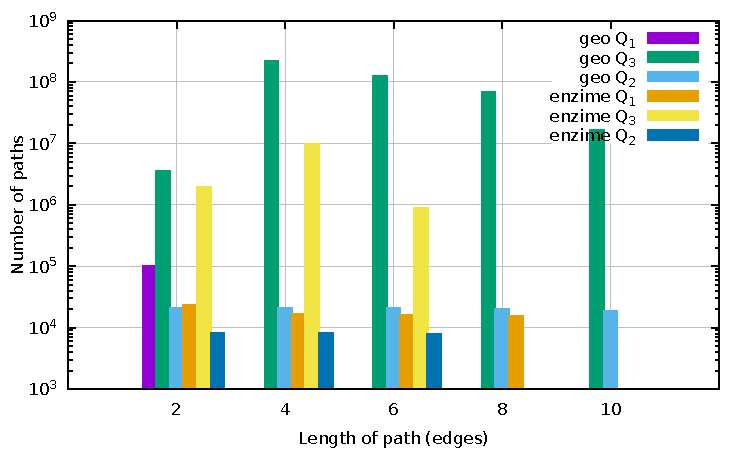
\includegraphics[width=0.5\textwidth]{data/path_per_length.pdf}
    \caption{Paths length destribution}\label{fig:pLength}
  \end{center}
\end{figure}

\begin{figure}[ht]
  \begin{center}
    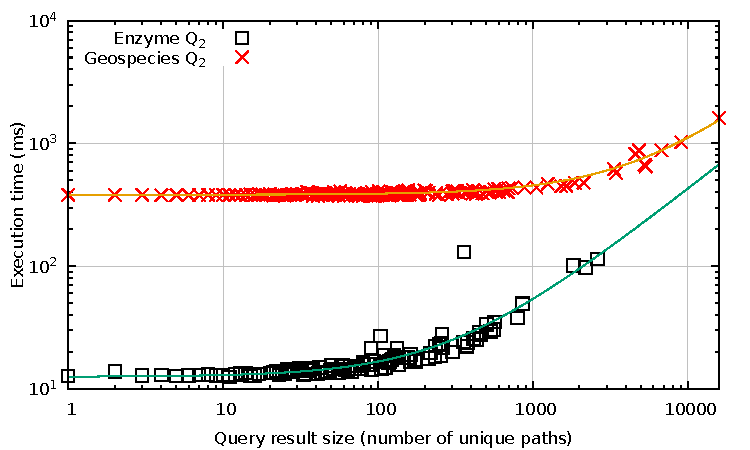
\includegraphics[width=0.5\textwidth]{data/time_per_paths_BT.pdf}
    \caption{Query execution time for $Q_2$ query and Enzime and Geospecies datasets}
    \label{fig:time_per_paths_BT}
  \end{center}
\end{figure}


First of all, we can see that provided datasets contain relatively short paths which satisfie queryes: longest patth contains 10 edges. 

Figures~\ref{fig:time_per_paths_BT},~\ref{fig:time_per_paths_NT} and~\ref{fig:time_per_paths_SCO} show dependency of query evaluation time on query answer size in terms of number of unique paths.
We calculate average time for answers with same size of answer.
First, we can see that query evaluation time is linear on answer size. 
Also we can see, that time which requred to evaluate query for one specific vertex is relatively small.
For example, for $Q_2$ and Enzime RDF 15051 queryes (99.75\%) were executed in less then 20ms, and only 3 quweryes requre more than 100ms. 

\begin{figure}[ht]
  \begin{center}
    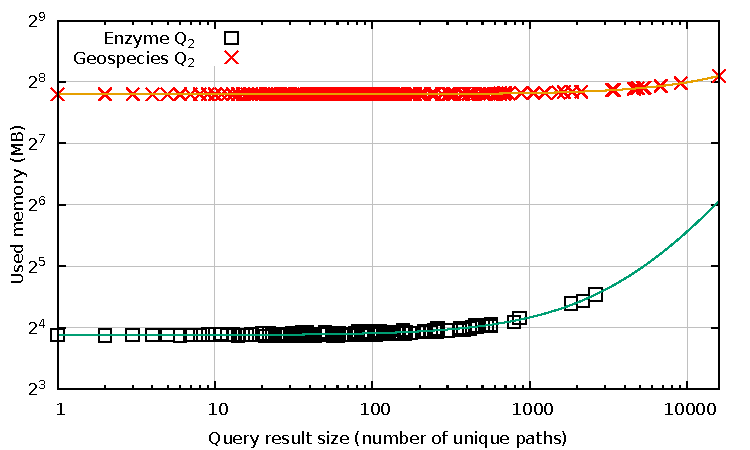
\includegraphics[width=0.5\textwidth]{data/mem_per_paths_BT.pdf}
    \caption{Query required memory for Enzime dataset}
    \label{fig:mem_per_paths_BT}
  \end{center}
\end{figure}

Figure~\ref{fig:enzime_mem_per_paths} shows dependency of memory requred to evaluate qurey on query answer size in terms of number of uniqie paths.

Finally, we can conclude that confext-free path querying in single source scenario can be efficiently evaluated by using !!! in case when number of paths in answer is big but its length is relatively small.
While all pairs scenario is still hard ~\cite{!!!}, single source scenarion, which is useful for manual or interactive data analysis, can be !!!
Also we can see that while theoretical time and space complexity of CFPQ algoritms at leas cubic, in demonstrated scenario real execution time and required memory is linear.
So, it is necessary to provide detailed time and space complexity analysis of algorithms.
